\chapter{TINJAUAN PUSTAKA}

\section{Hasil Penelitian Terdahulu}
Penelitian mengenai translasi isometri matematika geometri klasik ke geometri tropikal dan pelipatan tegar telah dibahas pada berbagai literatur. Ringkasan sintesis hasil penelitian terdahulu yang mendasari dan memotivasi riset tesis ini disajikan pada \ref{tab:penelitian_terdahulu}.

\bgroup
\renewcommand{\arraystretch}{1.5}
\begin{longtable}{|c|p{3.2cm}|c|p{8.5cm}|}
  \caption{Matriks Hasil Penelitian Terdahulu}
  \label{tab:penelitian_terdahulu} \\
  \hline
  \textbf{No} & \textbf{Peneliti}                  & \textbf{Tahun}                   & \textbf{Fokus \& Kontribusi Penelitian} \\
  \hline
  \endfirsthead
  
  \multicolumn{4}{c}%
  {{\thetable{} -- Lanjutan dari halaman sebelumnya}} \\
  \hline
  \textbf{No} & \textbf{Peneliti}                  & \textbf{Tahun}                   & \textbf{Fokus \& Kontribusi Penelitian} \\
  \hline
  \endhead
  
  \hline
  \endfoot
  
  \hline
  \endlastfoot
  
  1           & \citeauthor{mikhalkin2006tropical} & \citeyear{mikhalkin2006tropical} & Meletakkan fondasi awal dekuantisasi tropikal yang mereduksi polinomial kompleks menjadi fungsi linear secara \textit{piecewise}.                                          \\
  \hline
  2           & \citeauthor{hull2012project}       & \citeyear{hull2012project}       & Membakukan Teorema Kawasaki dan Maekawa untuk memodelkan kelayakan \textit{flat-foldable} secara klasik pada verteks origami tunggal.                                             \\
  \hline
  3           & \citeauthor{ku2014realization}     & \citeyear{ku2014realization}     & Melanjutkan teori \textit{rigid origami} dengan perumusan \textit{adjacency matrix} untuk merepresentasikan konektivitas antar engsel secara spasial.                                              \\
  \hline
  4           & \citeauthor{maclagan2015tropical}  & \citeyear{maclagan2015tropical}  & Mengonstruksi struktur \textit{tropical hypersurfaces} dan aljabar min-plus, menyediakan basis untuk konversi persamaan spasial ke ruang kombinatorik. \\
  \hline
  5           & \citeauthor{nekrasov2018geometry}  & \citeyear{nekrasov2018geometry}  & Merintis penggunaan teori tropikal pada dinamika spasial, menyingkap keterkaitan antara kurva origami spasial dengan Poligon Newton.                                  \\
  \hline
  6           & \citeauthor{zhang2018tropical}     & \citeyear{zhang2018tropical}     & Menunjukkan bahwa geometri tropikal min-plus murni bersifat isomorfis dengan mekanisme arsitektur ReLU pada \textit{Neural Network}.                                        \\
  \hline
  7           & \citeauthor{foster2020metric}      & \citeyear{foster2020metric}      & Mengevaluasi akurasi isometri dalam kurva tropikal menggunakan metrik Abel-Jacobi, menjamin keabsahan rentang deviasi galat dari kalkulasi rotasional.                                          \\
  \hline
  8           & \citeauthor{hayakawa2023analytical} & \citeyear{hayakawa2023analytical} & Menganalisis mekanisme infinitesimal tingkat kedua dari \textit{rigid origami}, menuntut kebutuhan mutlak akan penyelesaian sistem rotasi non-linear.                         \\
  \hline
  9           & \citeauthor{hayakawa2024rigid}     & \citeyear{hayakawa2024rigid}     & Memperluas studi sebelumnya pada struktur \textit{rigid grid} di mana hambatan \textit{loop closure} dan fenomena bifurkasi masif terjadi pada pola periodik.                             \\
  \hline
  10          & \citeauthor{bershadsky2024framework} & \citeyear{bershadsky2024framework} & Mendorong kerangka analitik pada tingkat fabrikasi riil (\textit{thick origami}), menyoroti urgensi atas simplifikasi efisien (seperti yang ditawarkan pada proposal ini).                      \\
\end{longtable}
\egroup

\section{Origami Matematis}
Matematika origami mempelajari batasan geometris dan kombinatoris dari selembar kertas yang dilipat tanpa disobek atau diregangkan. Pada pelipatan datar (\textit{flat folding}), keseluruhan kertas pada akhirnya dapat ditekan hingga rata di atas bidang dua dimensi \parencite{hull2012project}.

\subsection{Pola Lipatan}
Proses melipat kertas dapat diabstraksikan menjadi sebuah graf yang menempel pada selembar kertas datar. Graf ini memetakan jejak lipatan yang ditinggalkan saat kertas dibuka kembali.
\begin{definisi}
  Sebuah pola lipatan (\textit{crease pattern}) adalah sebuah graf planar yang diletakkan pada suatu daerah $D \subset \R^2$. Verteks dari graf tersebut disebut sebagai verteks origami, dan sisi (edge) dari graf tersebut disebut sebagai garis lipatan (\textit{creases}).
\end{definisi}

Pola lipatan pada sebuah verteks dikatakan dapat dilipat secara datar (\textit{flat-foldable}) jika panel-panel di sekitar verteks tersebut dapat dilipat hingga berhimpit pada satu bidang datar tanpa merobek kertas.

\subsection{Teorema Pelipatan Datar}
Dua teorema fundamental yang mengatur keseimbangan sudut dan garis lipatan pada satu titik verteks adalah Teorema Kawasaki dan Teorema Maekawa.
\begin{teorema}[Teorema Kawasaki]
  Misalkan $v$ adalah verteks tunggal di bagian dalam kertas dengan garis-garis lipatan yang bertemu di $v$ membentuk sudut-sudut $\alpha_1, \alpha_2, \ldots, \alpha_{2n}$ yang diurutkan secara sirkular. Pola lipatan di sekitar $v$ dapat dilipat datar (\textit{flat-foldable}) jika dan hanya jika jumlah sudut bolak-baliknya saling sama, yaitu:
  \[
    \alpha_1 + \alpha_3 + \ldots + \alpha_{2n-1} = \alpha_2 + \alpha_4 + \ldots + \alpha_{2n} = 180^\circ.
  \]
\end{teorema}

Setiap garis lipatan pada pola pelipatan diberi penugasan kelengkungan berupa Gunung ($M$, \textit{Mountain}) atau Lembah ($V$, \textit{Valley}).
\begin{teorema}[Teorema Maekawa]
  Misalkan $M$ adalah banyaknya jumlah garis gunung dan $V$ adalah banyaknya jumlah garis lembah yang bertemu pada satu verteks interior di kertas. Jika verteks tersebut dapat dilipat secara datar (\textit{flat-foldable}), maka selisih antara jumlah lipatan gunung dan lembah adalah $2$ atau $-2$. Secara matematis ditulis sebagai:
  \[
    M - V = \pm 2.
  \]
\end{teorema}

\begin{akibat}
  Berdasarkan Teorema Maekawa, jumlah derajat (\textit{degree}) atau banyaknya total garis lipatan pada setiap interior verteks pada pelipatan datar (\textit{flat folding}) pasti bernilai genap. Hal ini ditunjukkan oleh persamaan $M + V = (V \pm 2) + V = 2V \pm 2 \equiv 0 \pmod 2$.
\end{akibat}

\subsection{Matriks Ketetanggaan pada Graf Lipatan}
Karena pola lipatan pada dasarnya adalah graf planar, interaksi antar verteks dan panel dapat direpresentasikan secara aljabar linier menggunakan matriks ketetanggaan (\textit{adjacency matrix}).
\begin{definisi}
  Misalkan $G = (V, E)$ adalah graf planar lipatan dengan $n$ daerah panel. Matriks ketetanggaan $A$ berukuran $n \times n$ didefinisikan sebagai:
  \[
    A_{ij} = 
    \begin{cases}
      1, & \text{jika panel } i \text{ dan } j \text{ saling terhubung oleh satu garis lipatan}, \\
      0, & \text{lainnya}.
    \end{cases}
  \]
\end{definisi}
Representasi matriks ini amat esensial karena di dalam komputasi pelipatan, pencarian urutan jalur transformasi spasial antar-panel diselesaikan dengan melacak elemen matriks non-nol yang menunjukkan batas ketetanggaan atau konektivitas mekanis engsel \parencite{ku2014realization}.

\subsection{Teorema Justin dan Kondisi Non-Penetrasi}
Meskipun Teorema Kawasaki dan Maekawa memberikan jaminan bahwa suatu verteks secara lokal dapat ditekan hingga rata, teorema-teorema tersebut belum memperhitungkan fenomena tabrakan materi (\textit{self-intersection} atau penetrasi) pada panel-panel lipatan secara global. Pelipatan murni pada geometri nyata membutuhkan penugasan susunan panel (urutan \textit{layering}) yang konsisten dan saling kompatibel secara beruntun.

Untuk mengatasi ini, diperkenalkan Teorema Justin yang secara ketat mendefinisikan batas permutasi struktur dari tumpukan panel.
\begin{teorema}[Teorema Justin]
  Misalkan $v$ adalah verteks interior, dan setiap garis lipatan diberikan status gunung (M) atau lembah (V). Sebuah susunan tumpukan permukaan pada saat terlipat datar sepenuhnya dapat direpresentasikan oleh fungsi permutasi susunan $\sigma$. Susunan ini terhindar dari penetrasi mandiri jika dan hanya jika, untuk setiap pasang garis lipatan, paritas dari batas lipatan di antara kedua garis tersebut memenuhi ekuivalensi topologis pada pengurutan susunan $\sigma$.
\end{teorema}
Model analitik Justin menjadikan komputasi \textit{rigid folding} lebih dari sekadar perputaran sudut, melainkan sebuah penelusuran graf dalam ruang permutasi untuk memastikan panel kertas secara fisik tidak saling menembus saat ditekuk.

\subsection{Model Parametrik Miura-ori dan Kresling}
Untuk menguji dinamika pelipatan, struktur pola berulang atau teselasi periodik lazim digunakan. Dua struktur dasar yang paling luas dimanfaatkan pada meta-material adalah Miura-ori dan pola Kresling.

Pola Miura-ori dibangun dari paralellogram identik yang terhubung oleh ruas engsel lurus dengan satu derajat kebebasan mekanis (1-DOF). Persamaan relasi spasial kinematika dari pola Miura-ori dapat dituliskan berdasarkan sudut lipat internal $\theta$ dan sudut \textit{dihedral} di sepanjang engsel gunung/lembah. Hubungan antara kontraksi rasio panjang ruang spasial ($L_x, L_y$) terhadap bidang planar 2D murni dirumuskan secara analitik melalui ekspansi polinomial orde kedua, di mana geometri ini terbukti secara otomatis mempertahankan kekakuan struktur (rigiditas) di seluruh lintasan transformasi dari fase rata menuju silinder \parencite{hayakawa2024rigid}.

Di sisi lain, model Kresling sering diterapkan dalam perancangan elemen aktuator yang dapat ditekan (\textit{compressible}) dan struktur silinder origami. Berbeda dengan pola lurus pada Miura, Kresling memanfaatkan poligon segitiga transversal yang membengkokkan silinder melingkar dan menimbulkan pergerakan translasi sekaligus rotasi. Sifat ini dimanfaatkan secara radikal dalam membangun mekanisme infintesimal pada model origami tebal (\textit{thick origami}) yang harus mampu dilipat sepenuhnya ke dalam bangun datar dua dimensi \parencite{bershadsky2024framework}.

\section{Transformasi Spasial}
Dalam kinematika pelipatan kaku (\textit{rigid folding}), kertas direpresentasikan sebagai kumpulan panel polihedral (bidang datar) yang terhubung oleh engsel lurus berupa garis lipatan. Panel-panel ini dianggap sebagai benda tegar (\textit{rigid body}). Orientasi masing-masing panel ini dipetakan menggunakan transformasi Affine dalam ruang Euclidean $\R^3$.

\subsection{Transformasi Affine}
\begin{definisi}
  Suatu transformasi Affine pada ruang vektor $\R^n$ adalah suatu fungsi $f: \R^n \to \R^n$ yang dapat dinyatakan dalam bentuk
  \[
    f(\mathbf{x}) = A\mathbf{x} + \mathbf{b}
  \]
  di mana $A$ adalah pemetaan linear (berupa matriks berukuran $n \times n$) dan $\mathbf{b} \in \R^n$ adalah vektor translasi.
\end{definisi}
Dalam pemodelan origami lipatan kaku, titik asal (origin) diletakkan tepat pada engsel, sehingga vektor translasi $\mathbf{b} = \mathbf{0}$, menjadikan transformasinya murni didominasi oleh operasi rotasi spasial.

\subsection{Grup Ortogonal Khusus $SO(3)$}
Pemetaan linear rotasi di ruang $\R^3$ dilakukan oleh anggota dari Grup Ortogonal Khusus (Special Orthogonal Group).
\begin{definisi}
  Grup ortogonal khusus derajat 3, dinotasikan dengan $SO(3)$, adalah grup perkalian matriks rotasi berukuran $3 \times 3$ berisikan elemen bilangan riil. Himpunan ini didefinisikan sebagai:
  \[
    SO(3) = \{ R \in \R^{3 \times 3} \mid R^T R = I_3, \det(R) = 1 \}
  \]
\end{definisi}

\begin{contoh}
  Jika sebuah engsel (garis lipatan) berada di sumbu-$x$, rotasi sebuah panel dengan sudut $\theta$ di sekitar sumbu-$x$ dihitung dengan perkalian matriks rotasi $R_x(\theta) \in SO(3)$:
  \[
    R_x(\theta) =
    \begin{pmatrix}
      1 & 0          & 0           \\
      0 & \cos\theta & -\sin\theta \\
      0 & \sin\theta & \cos\theta
    \end{pmatrix}
  \]
\end{contoh}
Pergerakan dari panel pertama hingga panel terakhir yang mengitari satu verteks direpresentasikan oleh rantai perkalian sekuensial dari matriks-matriks $SO(3)$. Syarat \textit{loop closure} mengharuskan rantai perkalian ini kembali menjadi matriks identitas $I_3$. Operasi fungsi trigonometri berantai ini memicu latensi dan kompleksitas yang tinggi.

\subsection{Syarat Penutup Lengkung}
Transformasi spasial rotasi antar panel pada satu pola lipatan verteks tunggal (\textit{single vertex}) tidak terjadi secara independen. Terdapat sebuah batasan mekanis fisik bawaan yang mengharuskan bidang kertas tetap terhubung utuh mengitari verteks tanpa terjadi kerobekan.

\begin{teorema}[\textit{Loop Closure}]
  Misalkan suatu verteks tunggal dikelilingi secara sirkular oleh $k$ buah garis lipatan. Biarkan $R_1, R_2, \ldots, R_k \in SO(3)$ merepresentasikan matriks rotasi berantai yang melintasi setiap garis lipatan secara sekuensial. Agar kertas tetap bersambung, hasil komputasi perkalian dari serangkaian transformasi matriks tersebut wajib kembali ke orientasi awal mula, alias bernilai matriks identitas spasial:
  \[
    \prod_{i=1}^{k} R_i = R_1 R_2 \ldots R_k = I_3
  \]
\end{teorema}
Kondisi di atas dinamakan sebagai syarat \textit{Loop Closure Constraint}. Karena setiap matriks ortogonal $R_i$ memuat argumen fungsi sinus dan kosinus dari masing-masing sudut tekuk lipat (\textit{dihedral angle}), maka penyelesaian numeriknya memerlukan algoritma komputasi untuk menyelesaikan sistem persamaan trigonometri non-linear dengan orde komputasi tinggi. Studi literatur terbaru mengenai mekanisme infinitesimal tingkat kedua pada \textit{rigid origami} menunjukkan bahwa fenomena bifurkasi struktur spasial di sekitar kondisi ini menjadi subjek krusial dalam pergerakan dinamisnya \parencite{hayakawa2023analytical, hayakawa2024rigid}. Hal ini juga turut melatarbelakangi kebutuhan akan formulasi baru agar kendala engsel dan lipatan dapat diadaptasi untuk metode fabrikasi struktur material berskala tebal secara riil \parencite{bershadsky2024framework}.

\subsection{Parametrisasi Rotasi $SO(3)$ melalui Sudut Euler dan Quaternion}
Analisis pergerakan kontinu di atas memanifestasikan kebutuhan parametrisasi matriks rotasi $R \in SO(3)$ yang presisi. Pendekatan analitik konvensional sering memecah $R$ menggunakan sudut Euler, di mana rotasi spasial didekomposisi atas rotasi parsial mengelilingi tiga sumbu koordinat utama ($X, Y, Z$).

\begin{figure}[H]
  \centering
  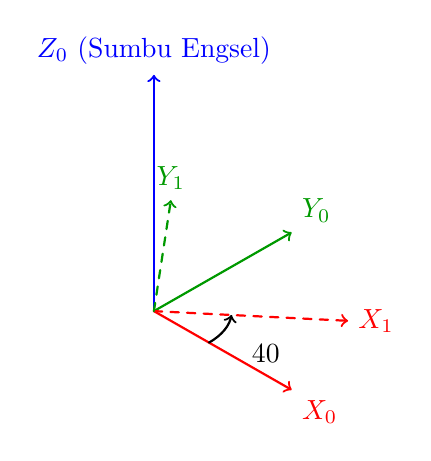
\begin{tikzpicture}[scale=2.5, line join=round, line cap=round]
    % Konfigurasi proyeksi 3D isometrik
    \tikzset{
      x={(0.7cm, -0.4cm)},
      y={(0.7cm, 0.4cm)},
      z={(0cm, 1cm)}
    }
    
    \coordinate (O) at (0,0,0);
    
    % Sumbu original (Frame 0)
    \draw[->, thick, red] (O) -- (1,0,0) node[below right] {$X_0$};
    \draw[->, thick, green!60!black] (O) -- (0,1,0) node[above right] {$Y_0$};
    \draw[->, thick, blue] (O) -- (0,0,1.2) node[above] {$Z_0$ (Sumbu Engsel)};
    
    % Sumbu rotasi (Frame 1) dirotasi sebesar theta
    \def\theta{40}
    \coordinate (X1) at ({cos(\theta)}, {sin(\theta)}, 0);
    \coordinate (Y1) at ({-sin(\theta)}, {cos(\theta)}, 0);
    
    \draw[->, thick, red, dashed] (O) -- (X1) node[right] {$X_1$};
    \draw[->, thick, green!60!black, dashed] (O) -- (Y1) node[above] {$Y_1$};
    
    % Arc sudut rotasi theta menggunakan segmen garis
    \draw[->, thick] (0.4, 0, 0) 
      \foreach \t in {5,10,...,35} {
        -- ({0.4*cos(\t)}, {0.4*sin(\t)}, 0)
      }
      -- ({0.4*cos(\theta)}, {0.4*sin(\theta)}, 0);
    
    \node[anchor=north west] at ({0.5*cos(\theta/2)}, {0.5*sin(\theta/2)}, 0) {$\theta$};
  \end{tikzpicture}
  \caption{Representasi Vektor pada Transformasi Rotasi $SO(3)$ di Seputar Engsel Origami.}
  \label{fig:kinematics}
\end{figure}

Kelemahan utama pemanfaatan sudut Euler pada pelipatan origami terletak pada fenomena \textit{gimbal lock}, yaitu di mana dua sumbu rotasi menjadi sejajar, mengakibatkan hilangnya satu derajat kebebasan komputasional. Oleh karenanya, formulasi matematika lanjut menggunakan bilangan kompleks empat dimensi bernama \textit{Quaternion} lebih diminati.
\begin{definisi}
  Suatu unit quaternion $\mathbf{q} = q_0 + q_1 \mathbf{i} + q_2 \mathbf{j} + q_3 \mathbf{k}$ dengan magnitudo $|\mathbf{q}| = 1$ secara kanonik berkorespondensi mutlak dengan suatu rotasi di $SO(3)$. Transformasi pada vektor $\mathbf{v} \in \R^3$ menggunakan unit quaternion ini dirumuskan lewat operasi perkalian Hamilton:
  \[
    \mathbf{v}' = \mathbf{q} \mathbf{v} \mathbf{q}^{-1}
  \]
\end{definisi}
Perkalian komutatif quaternion secara dramatis menghindari limitasi \textit{gimbal lock} dan menyederhanakan perhitungan sekuensial yang terjadi berulang-ulang di setiap engsel. Namun, hal ini tidak mengeliminasi sifat non-linear bawaannya.

\subsection{Model Kinematika Denavit-Hartenberg}
Dengan menjadikan setiap panel origami sebagai lengan tegar dan engselnya sebagai sendi putar murni (\textit{revolute joint}), model kinematika origami secara ekuivalen sepadan dengan struktur rantai robotika (\textit{robotic chain}). 
\begin{definisi}
  Parameter Denavit-Hartenberg (D-H) mendeskripsikan keterikatan ruang antar dua pasang engsel yang berurutan dalam kerangka spasial melalui konvensi empat matriks parameter absolut:
  \[
    A_i = \text{Rot}_z(\theta_i) \text{Trans}_z(d_i) \text{Trans}_x(a_i) \text{Rot}_x(\alpha_i)
  \]
  di mana $\theta_i$ merupakan sudut lipat engsel origami, dan $\alpha_i$ adalah sudut sektor panel.
\end{definisi}
Formulasi mekanika analitik D-H ini memperkuat abstraksi penyelesaian \textit{loop closure} ke tingkat di mana perkalian majemuk dari seluruh parameter ekuivalen dengan pembentukan sebuah lengkung kurva non-trivial berderajat jamak di ruang dimensi tinggi.

\section{Geometri Tropikal}
Sebagai alternatif, geometri tropikal akan digunakan untuk menyederhanakan perhitungan non-linear trigonometris yang rumit pada ruang kontinu menjadi perhitungan logis fungsi linear secara lokal \parencite{mikhalkin2006tropical}.

\subsection{Aljabar Min-Plus}
Geometri tropikal dibangun di atas landasan struktur semiring tropikal, dengan salah satu contoh utamanya adalah aljabar min-plus.
\begin{definisi}
  Aljabar min-plus adalah himpunan bilangan real yang diperluas $\R_{\min} = \R \cup \{\infty\}$ yang dilengkapi dengan dua operasi biner utama, yaitu operasi penjumlahan tropikal ($\oplus$) dan perkalian tropikal ($\otimes$):
  \begin{align*}
    a \oplus b  & = \min\{a, b\}, \quad \forall a, b \in \R_{\min} \\
    a \otimes b & = a + b, \quad \forall a, b \in \R_{\min}
  \end{align*}
  Elemen identitas untuk operasi $\oplus$ adalah $\infty$, dan elemen identitas untuk operasi $\otimes$ adalah $0$.
\end{definisi}
Sistem ini dinamakan semiring karena memenuhi sifat-sifat dasar gelanggang (ring) seperti komutatif dan distributif, namun tidak memiliki invers terhadap operasi penjumlahan $\oplus$.

\begin{contoh}
  Evaluasi operasi aritmetika pada semiring aljabar tropikal min-plus untuk bilangan skalar menghasilkan perhitungan berikut:
  \begin{align*}
    5 \oplus 7  & = \min(5, 7) = 5 \\
    5 \otimes 7 & = 5 + 7 = 12
  \end{align*}
\end{contoh}

\subsection{Fungsi \textit{Piecewise-Affine} Tropikal}
Dekuantisasi fungsi aljabar biasa menuju ranah semiring min-plus akan mereduksi kurva fungsi derajat tinggi menjadi sebuah kompleks fungsi linear sepotong-sepotong (\textit{piecewise-affine}).

\begin{definisi}
  Polinomial tropikal dalam $n$ variabel $x_1, \ldots, x_n$ adalah sebuah pemetaan fungsi $p: \R^n \to \R$ yang didefinisikan secara struktur min-plus sebagai:
  \[
    p(x_1, \ldots, x_n) = \bigoplus_{\mathbf{v} \in V} c_{\mathbf{v}} \otimes x_1^{\otimes v_1} \otimes \ldots \otimes x_n^{\otimes v_n}
  \]
  di mana $V \subset \Z_{\ge 0}^n$ adalah sebuah himpunan berhingga, dan $c_{\mathbf{v}} \in \R_{\min}$. Jika dijabarkan ke aljabar numerik standar, polinomial tropikal mendefinisikan fungsi konveks minimum yang bersifat \textit{piecewise-affine}:
  \[
    p(x) = \min_{\mathbf{v} \in V} \left( c_{\mathbf{v}} + \sum_{i=1}^n v_i x_i \right)
  \]
\end{definisi}

\subsection{Permukaan Tropikal dan Syarat Keseimbangan}
Polinomial fungsi nilai ekstrem minimum tropikal membentuk suatu topologi geometri spasial polihedral. Di dalam lanskap fungsi berdimensi jamak, sebuah kompleks permukaan di mana fungsi ini bersifat nondiferensiabel—yaitu daerah perpotongan di mana nilai minimum dicapai secara identik dan simultan oleh sedikitnya dua term affine—disebut sebagai permukaan hiper tropikal (\textit{tropical hypersurfaces}) \parencite{maclagan2015tropical}.

\begin{definisi}
  Suatu \textit{tropical hypersurface} $V(p)$ dari sebuah persamaan polinomial tropikal $p(\mathbf{x}) = \min_{\mathbf{v} \in V} \left( c_{\mathbf{v}} + \langle \mathbf{v}, \mathbf{x} \rangle \right)$ didefinisikan sebagai himpunan titik vektor $\mathbf{x} \in \R^n$ di mana batas nilai ekstrem minimum pada polinomial tersebut dicapai oleh minimal dua suku (\textit{term}) affine yang berbeda. 
\end{definisi}

Konsekuensi struktural yang lahir dari definisi tersebut adalah berlakunya hukum perimbangan pada tiap garis perpotongan.
\begin{teorema}[\textit{Balancing Condition}]
  Setiap titik persimpangan atau persambungan interior pada struktur \textit{tropical hypersurface} wajib memenuhi syarat kondisi perimbangan keseimbangan (\textit{balancing condition}). Untuk sebuah titik persimpangan verteks sebarang di dalam kerangka $V(p)$, suatu jumlahan berbobot (\textit{weighted sum}) dari serangkaian vektor arah (\textit{primitive integer vectors}) yang bertolak dari titik tersebut dan menyebar mengarah pada setiap sisi-sisi ketersambungan yang insiden dengannya, haruslah ekuivalen dan bernilai ekuilibrium nol:
  \[
    \sum_{j} w_j \cdot \mathbf{v}_j = \mathbf{0}
  \]
  di mana skalar $w_j \in \Z^+$ menyatakan bobot beban komputasi numerik (\textit{weight}) pada sisi lintasan ke-$j$.
\end{teorema}

Pada pemodelan \textit{rigid folding} origami yang diusulkan, \textit{loop closure constraint} dari transformasi isometri rotasi engsel engsel verteks kontinu akan diformulasikan ke dalam diskritisasi himpunan akar polinomial nilai-minimum tropikal menjadi \textit{tropical hypersurfaces}. Terdapat ekuivalensi yang kuat antara hukum perimbangan \textit{balancing condition} tropikal (di mana vektor-vektor yang bertolak dari simpangan berjumlah total nol) dengan Teorema Kawasaki dan Teorema Maekawa (penjumlahan dan perimbangan sudut lipatan gunung/lembah di titik pusat verteks interior). Oleh karenanya, kondisi struktural yang bersifat linear konveks ini bertindak secara sempurna menyulih peran non-linear konvensional dalam menjaga integritas jaring tata ruang pelipatan kertas secara utuh.

\subsection{Kurva Tropikal dan Poligon Newton}
Untuk dapat melakukan representasi visual terhadap interaksi suku-suku (terms) pada polinomial tropikal, parameter geometris konveks divisualisasikan dalam bentuk poligon batas.
\begin{definisi}
  Poligon Newton (\textit{Newton Polygon}), disimbolkan $\Delta(p)$, dari suatu fungsi polinomial tropikal dua variabel $p(x, y) = \bigoplus_{(i,j)} c_{i,j} \otimes x^{\otimes i} \otimes y^{\otimes j}$ adalah selubung cembung (\textit{convex hull}) dari seluruh kumpulan titik eksponen $(i,j)$ di dalam bidang dimensi-2 berkoordinat riil sedemikian sehingga koefisiennya bernilai terhingga ($c_{i,j} \ne \infty$).
\end{definisi}

Triangulasi dari Poligon Newton berkorespondensi langsung secara dual dengan konfigurasi kurva tropikal pada ruang nilai nyata. Garis-garis yang membentuk tulang punggung kurva tropikal senantiasa ortogonal secara topologis terhadap segmen garis triangulasi poligon Newton.

\begin{figure}[H]
  \centering
  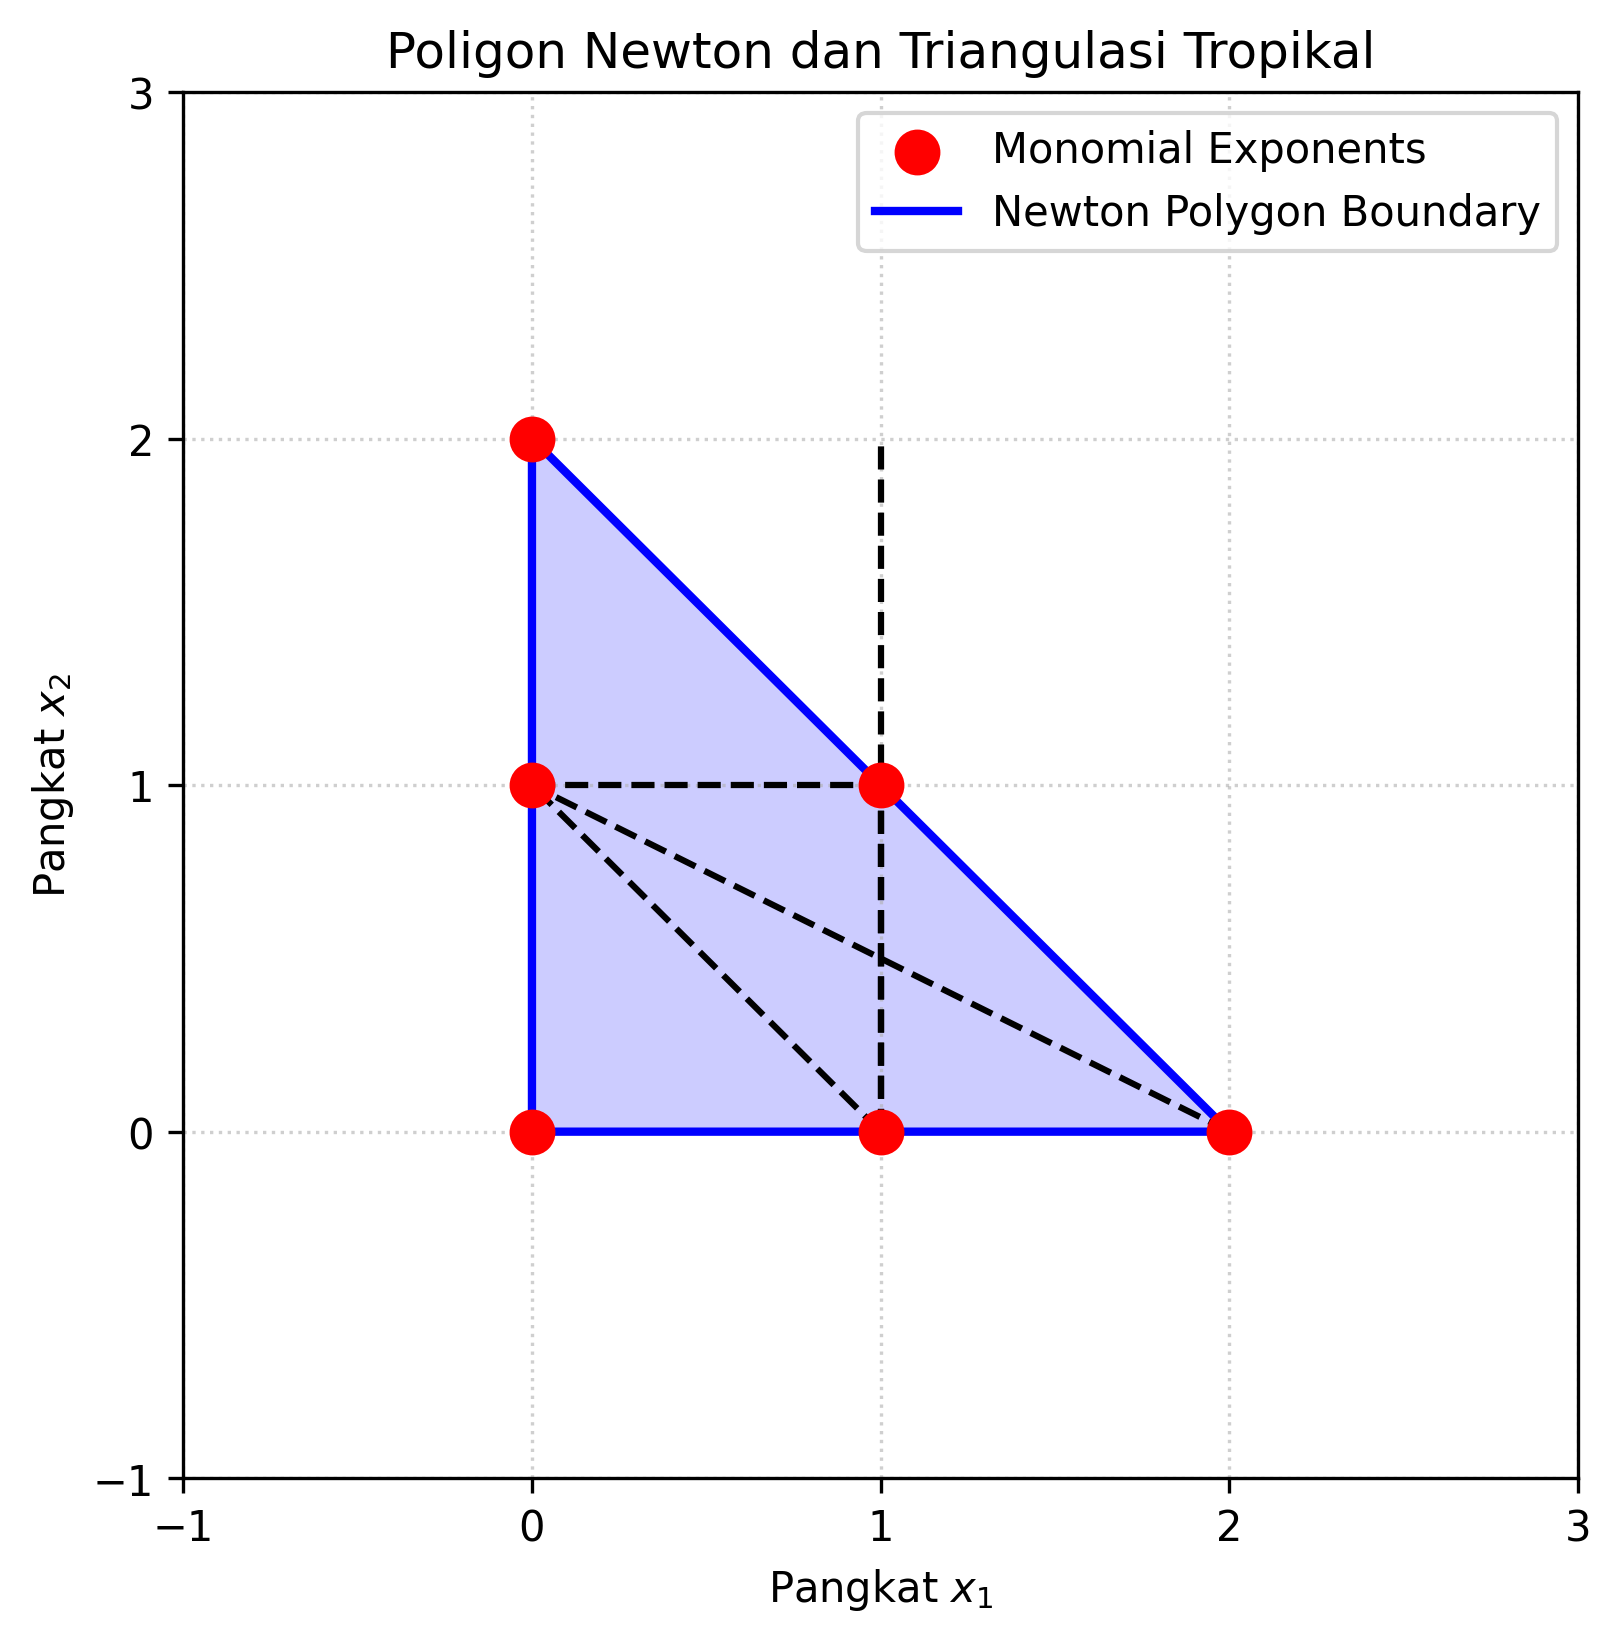
\includegraphics[width=0.55\textwidth]{foto/newton_polygon.png}
  \caption{Visualisasi Sebaran Batas Eksponen Monomial Pembentuk Poligon Newton Tropikal.}
  \label{fig:newton_polygon}
\end{figure}

Sifat korelasi dualitas struktur kombinatorik ini memberikan fleksibilitas komputasi yang menjanjikan, di mana manipulasi topologis fungsi polinomial dapat diproyeksikan langsung terhadap titik-titik diskret pada ruang eksponennya yang linear tanpa perlu menggunakan metode komputasi matriks \textit{floating point} non-linear rumit layaknya pada struktur spasial trigonometri $SO(3)$.

\subsection{Teorema Kapranov}
Alasan mendasar mengapa pergerakan isometri origami dapat dialihbahasakan ke semiring tropikal adalah landasan fundamental geometri tropikal yang dikenal sebagai Teorema Kapranov.
\begin{teorema}[Teorema Kapranov]
  Untuk sebarang himpunan bilangan riil pada polinomial atas ruang Puiseux (aljabar terstruktur metrik diskret), \textit{tropical hypersurface} $V(p)$ dari ideal polinomial $p$ sama halnya dengan penutupan dari ruang limit evaluasi nilai (valuation) atas persimpangan semua titik akar dari varietas aljabarnya secara klasik.
\end{teorema}
Keterikatan absolut ini membuktikan jaminan matematis secara pasti bahwa kalkulasi minimum polinomial tropikal pada matriks ketetanggaan origami, meskipun terlihat sangat diskret dan dipenuhi persamaan garis kaku (\textit{piecewise}), secara akurat tetap menyajikan bayangan presisi penuh atas gerakan membelok kontinu ruang spasial origami. Hal ini juga menjadi landasan pengukuran isometri menggunakan pemetaan metrik Abel-Jacobi, menjamin keabsahan jarak rotasional \parencite{foster2020metric}.

\subsection{Arsitektur Tropikal pada Jaringan Saraf Tiruan}
Jaringan saraf tiruan mendalam (\textit{Deep Neural Networks}), secara khusus arsitektur berlapis maju (\textit{feedforward}) yang didorong oleh fungsi aktivasi ReLU (\textit{Rectified Linear Unit}), memiliki sifat yang secara intrinsik ekuivalen terhadap semiring tropikal. Karakteristik ini membuka gerbang bagi formulasi konvergensi optimasi lintasan (\textit{path planning}) algoritma origami pada komputasi cerdas (AI) \parencite{zhang2018tropical}.

Fungsi aktivasi ReLU didefinisikan secara matematis murni sebagai pencarian nilai keabstrakan ekstrem, yaitu $f(x) = \max(0, x)$. Bentuk perhitungan maksimum affine ini adalah cerminan kembar berbalik dari persamaan aljabar min-plus, menjadikannya satu entitas kesatuan bersama dengan dekuantisasi \textit{piecewise-affine} tropikal. 

\begin{figure}[H]
  \centering
  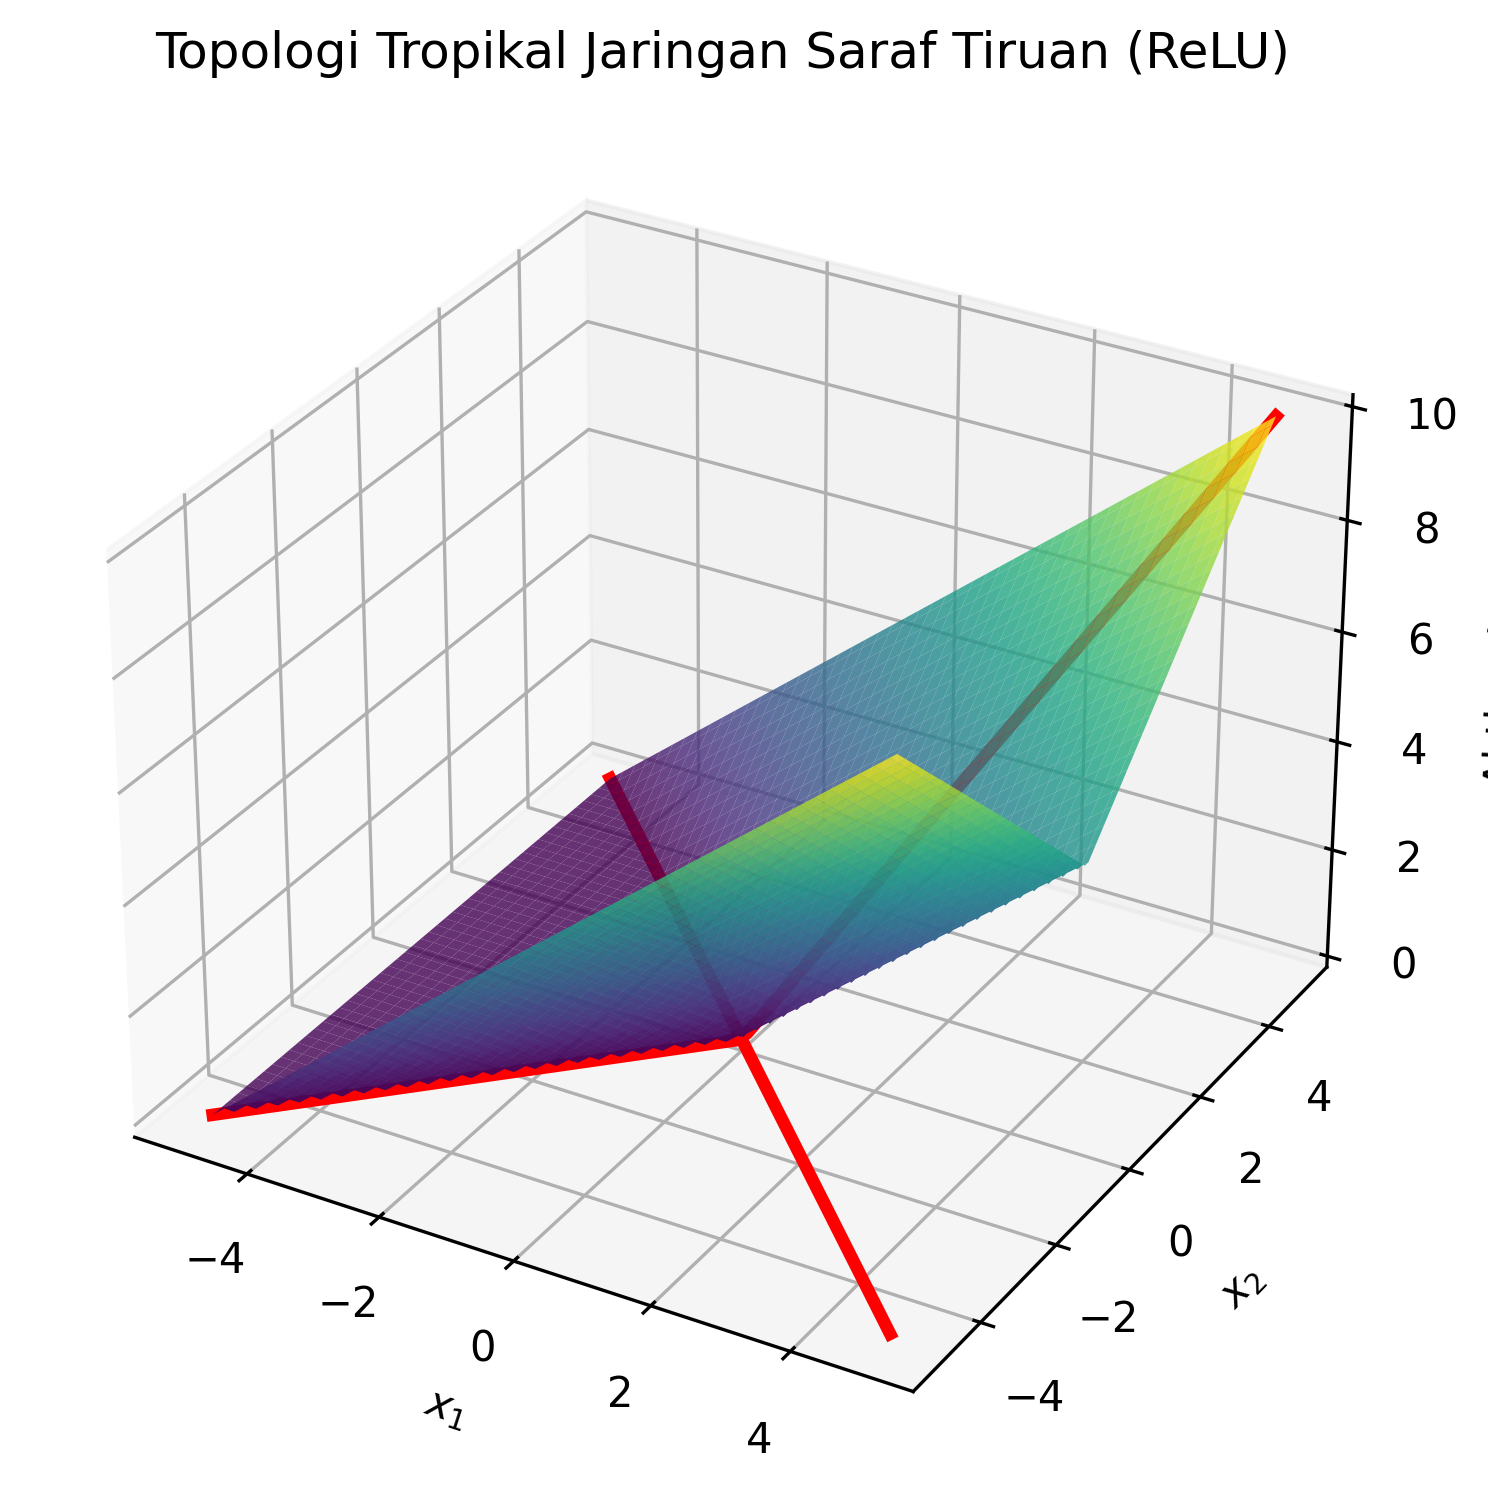
\includegraphics[width=0.6\textwidth]{foto/tropical_neural_network.png}
  \caption{Topologi Batas Keputusan dari Konstruksi Neural Network ReLU sebagai Entitas \textit{Tropical Hypersurface} Berdimensi Ruang Spasial Tiga (3D).}
  \label{fig:tropical_nn}
\end{figure}

Setiap parameter \textit{hidden layer} saraf tiruan merupakan dekomposisi \textit{tropical hypersurface} berdimensi jamak. Oleh sebab itu, fungsi kerugian optimasi \textit{loss surface} suatu AI untuk menyelesaikan pencarian pola kombinasi \textit{crease pattern} ideal untuk transformasi \textit{rigid folding} sejatinya sedang mengomputasi batasan lintasan dalam batas konveks poligon Newton. Implementasi AI tak sekadar berfungsi layaknya fungsi "hitam" konvensional, melainkan bertindak bak orkestrasi pergerakan \textit{Newton Polygon} di ranah geometri min-plus murni secara geometris riil \parencite{nekrasov2018geometry}.